\chapter{Introduction}
\label{chap:Intro}

The abstract form of fluids in the natural world has inspired artists and scientists for centuries. 
For instance, in through careful experimentation, Leonardo da Vinci (1452--1519), besides studying water from an artistic perspective, also discovered the law of conservation of mass for incompressible one-dimensional flows \cite{gad1998fluid}. A myriad of impressionistic works such as Hokusai's {\em The Great Wave off Kanagawa} (1829--1833), van Gogh's {\em The Starry Night} (1889), Monet's {\em Water Lilies} (1897--1926), and many others draw inspiration from the variety of moods that water and air express, capturing destruction, abstraction, and serenity, all with their still images. In the sonic arts, composers such as Debussy and Ravel explored the unfolding undulations of fluids over time in a way that visual artists could not, composing impressionistic pieces such as {\em Une barque}, {\em La Mer}, {\em Reflets dans l'eau}, {\em Le vent dans la plaine}, and {\em Jeux d'eau}. Through their harmonic and rhythmic language, these pieces abstractly depict the variety of moods that fluids can express, from turbulent spray to calm stillness. However, a formal interplay between a particular time-evolving process of fluid dynamics and time-evolving sound is not present. Such formal approaches to generating art were not explored until the twentieth century.

The Greek composer and architect, Iannis Xenakis (1922--2001), was an early pioneer of the use of mathematical processes in music composition. Two of his compositions, {\em Pithoprakta} (1955--56) and {\em N'Shima} (1975) relied on mathematical processes derived from the statistical mechanics of gases on a molecular level. His magnum opus, {\em Formalized Music: Thought and Mathematics in Music} \cite{xenakis1992formalized}, expounds his aesthetic philosophy as well as his techniques for composing music stochastically through mathematical processes. Many other composers and researchers followed up in the direction of algorithmic
composition, albeit with their own individual aesthetic goals, including Karlheinz Stockhausen, Max Mathews, John Chowning, and John Cage.

In the visual arts, more powerful computing and research into computer graphics eventually led to the area of physics-based fluid animation. Early research in the field of computational fluid dynamics and mechanical engineering in the 1960s became translated into the domain of computer graphics starting in the 1990s. Work by O'Brien, Fedkiw, Bridson, Stam, Treuille, and others paved the way for many different types of fluid animation, ranging from real-time, simplistic effects suitable for computer games, to photorealistic renders for films. A large body of work has been dedicated to improving the efficiency of these physics-based simulations, including
fluid-implicit particle methods (FLIP), spatial coarsening methods, position-based methods, and vortex-sheet methods. \cite{brackbill1988flip, Ando:2013:HAL, Macklin:2014, Pfa12}

The experiment of Ernst Chladni (1756--1827), involving the patterns of sand accumulating on the surface of vibrating metal plates, was an early audiovisual link between visual shape and sonic frequency. Using a violin bow to vibrationally excite a metal plate covered with sand, Chladni observed a variety of intriguing nodal patterns, depending on the shape of the plate as well as the frequency of the vibration. The Swiss scientist Hans Jenny (1904--1972) pioneered the general study of this principle of visual patterns (as in Figure \ref{fig:cymatics}) associated with sonic vibrations, which he named ``Cymatics.'' Many composers and artists followed in the footsteps of Jenny, including Alvin Lucier, Gy{\"o}ray Kepes, and Alexander Lauterwasser. 

\begin{figure}
\centering
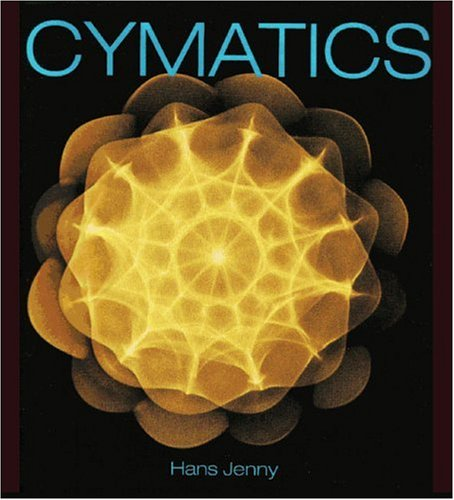
\includegraphics[width=0.5\textwidth]{chap1/figures/cymatics.jpg}
\caption{\em One of the visual patterns from Hans Jenny's seminal text.}
\label{fig:cymatics}
\end{figure}

This dissertation serves as a bridge between generative art and sound, computer graphics, and cymatics. Using computational fluid dynamics simulations as our background data, we define a bridge between the visual
and sonic results in the spirit of cymatics, linking resonant visual shapes of vibration to their corresponding audio frequencies. Along the way, we devise a data compression algorithm as part of the simulation pipeline to
ease the computational load. 

\section{Systems of Sonification and Aesthetic Goals}
The term ``sonification'' has many subtly different interpretations and definitions, but we use it in this dissertation to refer broadly to the association of data to sound. Scientifically-focused sonifications can reveal underlying
qualitative patterns of the data, while artistic-focused sonifications can serve as a framework for composing novel musical or even audiovisual works. In this dissertation, we use the phenomenon of fluid dynamics as our
data, focusing on a system of sonification that, while revealing certain qualitative features of the fluid motion, mostly serves to generate novel audiovisual pieces. More precisely, we use the the {\em subspace} method of simulation, based on a stable computational fluid dynamics simulation, as our data, and a model-based sonification system to associate the data with musical sound, in analogy with the resonant modal shapes and 
frequencies as discovered by Chladni and Jenny in the field of cymatics.

\section{Data Compression and Memory Obstacles with Subspace Matrices}
The general technique of data compression began with Claude Shannon and the field of information theory. It is of practical relevance for many problems in computing, as reducing memory footprints
can make certain simulations more feasible to run. The general idea of data compression is that by exploiting patterns or redundancies in data, we can often represent the same data in a more terse form.
A wide variety of research in this area has produced many successful compression schemes, from lossless compression of arbitrary files (ZIP) to lossy compression of image (JPEG), audio (MP3), and video (MPEG).

The subspace method of simulation, while known to achieve large speedups over regular full-space simulations, also requires a potentially prohibitive memory cost, consuming dozens of gigabytes of RAM 
in high-resolution, three-dimensional simulations. While other research has been done on compressing blendshape matrices for facial animations and eigenmode matrices for modal sound synthesis,
to our knowledge, no previous work on compressing fluid subspace matrices has been done.

\section{Thesis Statement and Main Results}
The thesis statement is as follows:

\begin{addmargin}[1em]{2em}
{\em The method of subspaces in computational fluid dynamics for computer graphics can be leveraged to systematically produce artistic audiovisual pieces.}
\end{addmargin}
In particular, I demonstrate three main results:

\begin{itemize}
	\item I propose a versatile system of sonification of fluid subspaces.
	\item I describe a data compression algorithm for fluid subspaces to help ease high computational costs.
	\item I demonstrate the sonification system with several audiovisual {\'e}tudes.
\end{itemize}

The first result, the sonification system, achieves a two-way coupling between sound and visual, allowing the visual to drive the sound, the sound to drive the visual, or even a third intermediary process to govern both the sound and visual simultaneously. The flexibility of the system allows the composer to generate a variety of sounds and visual forms that are nonetheless intertwined in a common language. 

The second result, the data compression algorithm, achieves an order of magnitude compression of fluid subpsace matrices needed in memory during runtime without any perceivable visual artifacts. The main result is the technique behind the compression scheme, a transform-based algorithm, combined with a novel sparse frequency-domain projection and reconstruction.

The third result, the audiovisual {\'e}tudes, serve as proof of concept of the possibility of the sonification system as a means toward developing an audiovisual language. Carefully chosen parameters are modulated to demonstrate compositional gestures that can be achieved in both the audio and visual domain. 

\section{Organization}
The dissertation is organized as follows. Chapter \ref{chap:chap2} provides background and related work in the domain of generative art and sonification. Chapter \ref{chap:chap3} gives additional background in the domain of fluid simulation for computer graphics, focusing in particular on the method of subspaces. Chapter \ref{chap:chap4} describes the data compression algorithm for fluid subspaces and shows its effectiveness on a variety of different subspace simulations. In Chapter \ref{chap:chap5} we describe the system of sonification of the fluid subspaces. Chapter \ref{chap:chap6} demonstrates the versatility of the sonification system through a series of systematic audiovisual {\'e}tudes. Finally, Chapter \ref{chap:chap7} presents conclusions and directions for future work.
